\section{Risikoabsch�tzung}
\begin{itemize}
\item Schnittstelle Lotus Notes
\item Termin: Das Projekt wird nicht zum vereinbarten Termin abgeschlossen.
\item Qualit�t: Die vereinbarten Anforderungen werden nicht erf�llt.
\item Budget: Das Projekt wird teurer als geplant.
\item Einzigartigkeit, das Projekt beinhaltet wenigstens einige Elemente, die noch nie zuvor so gemacht wurden.
\item Komplexit�t ist vielfach vorhanden, wie z.B. im technischen oder wirtschaftlichen Bereich, von den Schnittstellen her gesehen oder aber wegen der relationalen Einbindung eines Projektes.
\item Annahmen und Einschr�nkungen bzgl. der zuk�nftigen Entwicklung, sowohl ausgesprochen (offen) als auch implizit (versteckt), die sich als falsch erweisen k�nnen.
\item Ziele, die die Ma�nahmen nach sich ziehen und f�r den Erfolg eines Projektes ma�geblich sind, sind in der Regel fest definiert und manchmal auch widerspr�chlich.
\item Menschen, wie z.B. die Projektteam-Mitglieder und das Management, Kunden, Lieferanten und Subunternehmer sind alle zu einem gewissen Ma� unberechenbar.
\item Anforderungen der Stakeholder, Erwartungen und Ziele k�nnen sich ver�ndern, �berlappen oder manchmal auch widersprechen.
\item Ver�nderungen, denn jedes Projekt ver�ndert und bewegt etwas aus der bekannten Gegenwart in eine unbekannte Zukunft hinein.
\item Umfeld, in dem jedes Projekt existiert, sowohl das interne organisatorische Umfeld als auch das externe Umfeld, in dem Ver�nderungen passieren k�nnen, die der Steuerung des Projektes entzogen sind.
\end{itemize}

\subsection{Risiko - Eintrittswahrscheinlichkeit - Schadenpotenzial}

%\begin{center}
%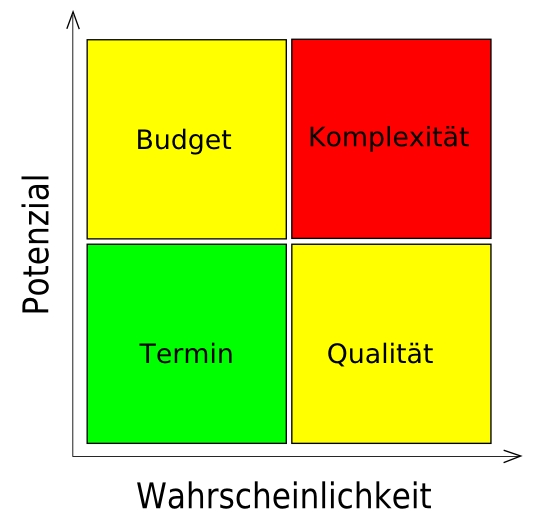
\includegraphics[width=0.8\textwidth]{abbildungen/Wahrscheinlichkeit-Potenzial.eps}
%\end{center}

\subsection{Risikomatrix}
\subsection{Vorbeugema�nahmen}
\subsection{Korrekturma�nahmen}